\section{Interface-Closed Recovery}
\label{sec:interface-repair}
\subsection{Bidirectional Repair Closure}
A replacement propagates two kinds of obligations. If its output is
incompatible with an unchanged consumer, that consumer must enter the region.
Conversely, a replaced consumer may reject an unchanged predecessor's output,
requiring that predecessor to enter. Construct the implication relation
\begin{equation}
\begin{split}
 u\Rightarrow v &\quad\text{if }(u,v)\in E\land\neg C^{\rho}_{uv}(1,0)\\
 v\Rightarrow u &\quad\text{if }(u,v)\in E\land\neg C^{\rho}_{uv}(0,1)
\end{split}
\end{equation}
Starting with $R_0=F$, compute
\begin{equation}
 R_{k+1}=R_k\cup\{v:\exists u\in R_k,\ u\Rightarrow v\}
 \label{eq:repair-closure}
\end{equation}
This inflationary monotone operator reaches a fixed point $R^*_{\rho}$ on a finite
graph. The worklist records the implication responsible for every added node,
providing a checkable explanation of the repair region.
Figure~\ref{fig:repair-obligations} illustrates both propagation directions
and an immutable-boundary conflict.

\begin{figure}[t]
\centering
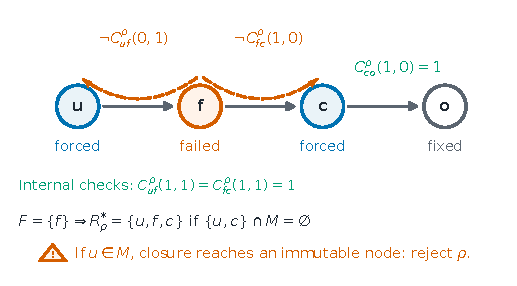
\includegraphics[width=\columnwidth]{figures/repair_obligations.pdf}
\caption{Bidirectional closure and feasibility checks.}
\label{fig:repair-obligations}
\end{figure}

\textbf{Theorem 1 (least feasible region).}
For a fixed replacement assignment $\rho$ and its Boolean compatibility relation, if
$R^*_{\rho}\cap M=\varnothing$ and every edge $(u,v)$ internal to $R^*_{\rho}$ satisfies
$C^{\rho}_{uv}(1,1)$,
then $R^*_{\rho}$ is the unique inclusion-least feasible region. Otherwise no feasible
region exists for that assignment.

Every feasible region contains $F$ and is closed under each forced implication,
so it contains $R^*_{\rho}$. Edges $(u,v)$ with both endpoints outside retain
$C^{\rho}_{uv}(0,0)$; closure checks
mixed edges, and the final test checks internal edges.

It follows that $R^*_{\rho}$ minimizes any nonnegative additive node-change cost for
the fixed assignment. A worklist examines each node once and each edge at most
twice, taking $O(|V|+|E|)$ time after compatibility is available. Enumerating a
finite assignment set $\mathcal{A}$ and choosing its smallest feasible closure
is exact over $\mathcal{A}$; the cost of discovering that set is separate.

\textbf{Theorem 2 (contextual interface preservation).}
When compatibility predicates are sound for the port contracts, replacing
exactly the nodes of a feasible $R^*_{\rho}$ preserves all interfaces of the unchanged
context. Consider an acyclic workflow whose tools are deterministic functions
of their explicit inputs, share no hidden mutable state, honor the same declared
failure semantics, and execute unchanged nodes in their original topological
order. The resulting dataflow remains well typed. If the replacement also
preserves every normalized value exposed at the repair boundary, the unchanged
continuation produces the same observable suffix outputs.

Every edge is original--original, mixed, or replacement--replacement;
the original contract, closure, or final test checks each case, respectively.
Topological induction then propagates valid types, and matching exposed
values preserves the deterministic suffix.

These properties identify when single-call substitution is insufficient:
if $\neg C^{\rho}_{fc}(1,0)$, every feasible repair containing the failed producer
$f$ must also include consumer $c$. The boundary, rather than a fixed repair
depth, determines where repair may stop. The guarantees concern interface
composition; functional eligibility must be supplied separately.

\subsection{Joint Choice and Scope}
Fixed-assignment closure does not select implementations. Let $A_v$ contain
node $v$'s original $0_v$ and operation-equivalent alternatives; eligibility
is checked before interface optimization. Let $c_v(s)\geq0$ be choice cost,
$c_v(0_v)=0$, and $\Gamma_{uv}(s,t)$ denote edge compatibility.
The joint decision is
\begin{equation}
\begin{split}
\min_{x_v\in A_v}\quad &\sum_{v\in V}c_v(x_v)\\
\text{s.t.}\quad &x_f\ne0_f\ (f\in F)\quad x_m=0_m\ (m\in M)\\
&\Gamma_{uv}(x_u,x_v)=1\quad((u,v)\in E)
\end{split}\label{eq:joint-choice}
\end{equation}
Source and sink ports remain immutable. Assignment $\vec{x}=(x_v)$ changes
region $R(\vec{x})=\{v:x_v\ne0_v\}$; the cheapest seed need not minimize
total repair cost. Theorems~3 and~4 solve this structural objective; context
and value admission then filter the resulting programs.

For a forest, root each underlying undirected component arbitrarily. For a
tree parent $v$ and child $w$, let $B_{vw}(s,t)=\Gamma_{vw}(s,t)$ when
$(v,w)\in E$, and $B_{vw}(s,t)=\Gamma_{wv}(t,s)$ otherwise. Thus $B$ always
orders its arguments as parent then child while preserving dataflow direction.
Let $D_v(s)$ be the minimum cost of the subtree below $v$ conditional on
$x_v=s$. For child $w$,
\begin{equation}
D_v(s)=c_v(s)+\sum_{w\in\mathrm{ch}(v)}
\min_{t\in A_w:\,B_{vw}(s,t)=1}D_w(t)
\label{eq:joint-dp}
\end{equation}
where an empty minimum is $+\infty$. Ineligible choices have infinite cost. Backtracking
from the minimum root state returns both selected implementations and
$R(\vec{x})$.

\textbf{Theorem 3 (exact joint repair on forests).}
Equation~\eqref{eq:joint-dp} returns a globally minimum-cost assignment
satisfying~\eqref{eq:joint-choice}, or reports infeasibility. With $k_v=|A_v|$,
it takes $O(\sum_{(u,v)\in E}k_uk_v+\sum_v k_v)$ time and
$O(\sum_v k_v)$ score states; storing backpointers additionally uses
$O(\sum_{(v,w):w\in\mathrm{ch}(v)}k_v)$ memory.

\emph{Proof.} Conditional on $x_v=s$, child subtrees are independent;
leaf-to-root induction makes $D_v(s)$ their optimum. Minimizing each root
gives the global optimum or infeasibility. Edge option pairs and states give
the stated bounds.\hfill$\square$

Algorithm~\ref{alg:joint-repair} summarizes the exact forest procedure and its
returned assignment and region.

\begin{algorithm}[!b]
\caption{\textsc{ExactJointRepair} on a forest}
\label{alg:joint-repair}
\footnotesize
\begin{algorithmic}[1]
\REQUIRE Rooted forest $G$; choices $\{A_v\}$; costs $\{c_v\}$;
compatibility $\Gamma$; failed nodes $F$; immutable nodes $M$
\ENSURE Minimum-cost $(\vec{x}^{*},R(\vec{x}^{*}))$, or
\textsc{infeasible}
\STATE Remove original choices at failed nodes and nonoriginal choices at
immutable nodes
\STATE Remove choices that violate immutable source or sink ports
\STATE For each $v$ in postorder and $s\in A_v$, compute $D_v(s)$
by~\eqref{eq:joint-dp}
\IF{some root has no finite state}
  \RETURN \textsc{infeasible}
\ENDIF
\STATE Backtrack the minimizing states
\RETURN $(\vec{x}^{*},R(\vec{x}^{*}))$
\end{algorithmic}
\end{algorithm}

For multi-input DAGs, port-bound edges yield pairwise compatibility factors.
Min-sum variable elimination~\cite{dechter1999bucket} with min-fill ordering
and backpointers extends exact repair to shared consumers.

\textbf{Theorem 4 (bounded-width joint repair).}
For a port-bound workflow whose induced elimination width is $w$ and whose
nodes have at most $k$ eligible implementations, min-sum variable elimination
solves~\eqref{eq:joint-choice} exactly in
$O((|V|+|E|)k^{w+1})$ time and
$O(|V|k^w+|E|k^2)$ memory including the original pairwise factors,
or reports infeasibility.
Elimination preserves separator optima; temporary factors have at most $w+1$
variables, and backtracking attains the optimum. Forests have width one.

With arbitrary supplied pairwise compatibility predicates, deciding whether
any joint repair exists is nondeterministic polynomial-time (NP)-complete even when the dependency graph is a
DAG and each failed node has only three eligible replacements: orient a
3-coloring instance acyclically and make adjacent replacement colors
incompatible. Bounded width therefore gives a tractable exact class.


\subsection{Compiling Local Recovery Programs}
The compiler constructs a local graph $i\to f\to c\to o$, where $f$ is the
failed producer, $c$ a catalog-linked continuation, and $i,o$ immutable input
and output ports. For each alternative producer and consumer in the same
respective public categories and domains, it constructs a compatibility table
and invokes the fixed-point closure with $F=\{f\}$ and $M=\{i,o\}$. Enumeration includes
the original consumer and does not prefilter on internal or output-boundary
compatibility. Closure therefore determines whether to retain $c$, replace
it, or reject the assignment.

Three evidence tests instantiate this table. The input edge requires a
lossless transport of the observed failed-call arguments. The internal edge
uses nominal producer references and a unique payload projection for each
old--new combination. The output edge requires the chosen consumer's
normalized public output schema to equal the original boundary. The compiler
stores every forced inclusion and rejection alongside the emitted program.
It emits only the nodes chosen by closure as replacements; an unchanged
consumer can still execute as the continuation.

\textbf{Corollary (local structural admission).}
If the alternative producer cannot bind to the original consumer, then a
candidate is structurally admitted exactly when concrete input transport, alternative-pair
binding, and output-boundary preservation all hold. Its least region is
$\{f,c\}$. Otherwise, a valid input transport admits the producer-only region
$\{f\}$ with the original consumer. Function, context, and boundary-value gates are
applied after this structural test.

With $f$ forced and the ports immutable, an incompatible original consumer
forces $c$ into the region. The three evidence tests then check precisely its
input, internal, and output boundaries.

Theorem~1 applies exactly to this Boolean structural relation. Nominal
annotations establish payload identity for interface checking; the separate
boundary-value predicate establishes semantic eligibility. Concrete input validation
checks the selected dataflow at execution time. Theorem~2 gives the typing
guarantee under sound application port contracts.

Each candidate exposes a function whose arguments contain only the context
still needed from the model. After selection, the executor invokes the
producer, binds its actual successful output into the consumer, validates
the resulting input, and invokes the consumer. A failed producer interrupts
the program before the consumer is dispatched. The original failure and both
recovery invocations remain in the execution trace. This separates semantic
choice from deterministic dataflow binding.

\subsection{Recovery Packet and Authority Boundary}
At an observed failure record $\xi$ containing failed input $a$, let
$\mathcal{P}(\xi)$ be the locally compiled interface-closed programs. A declared
operation relation $\sim_{\mathrm{op}}$ admits a
replacement only when its producer and consumer retain the respective
operations of the failed call and intended continuation. In the relational
instantiation, this requires the same source--target projection signature;
$\Phi$ below supplies the input-specific value evidence. At program level,
$K(p,\xi)$ returns context assembled from
observed arguments, public defaults, and explicit task fields, and
$K(p,\xi)=\bot$ when that context does not validate against the program's public
input schema. The boundary-value predicate $\Phi(p,a)$ accepts a program only
when its returned value is certified at the observed input. The dispatch set is
\begin{equation}
\begin{aligned}
\mathcal{D}(\xi)=\{p\in\mathcal{P}(\xi):\;&
p\sim_{\mathrm{op}}\xi\ \land\ K(p,\xi)\ne\bot\\
&{}\land\ \Phi(p,a)=1\}
\end{aligned}
\label{eq:dispatch-set}
\end{equation}
The recovery packet records an admitted program, its validated inputs,
interface boundary, and boundary-value evidence. The advice policy returns the packet
to the model; the dispatch policy executes the sole member when
$|\mathcal{D}(\xi)|=1$ and otherwise returns the candidates. Context extraction copies matching failed-call arguments, uses
public schema defaults, and recognizes explicit priority or channel in the
user request. It never reads benchmark reference paths or judge labels.

\textbf{Proposition (choice collapse).} Conditional on a sound operation
relation, sound interface and boundary-value predicates, valid context, and a non-committing failed
call, if $\mathcal{D}(\xi)=\{p\}$, every recovery restricted to the declared
operation-equivalent, context-valid, value-certified local program class
selects $p$. Executing $p$
preserves the unchanged dataflow boundary; its consumer receives a projection
of the observed producer result, not a predicted value.

Within the declared local class, this rule removes a determined choice from
the model's action space; ambiguous or uncertified recovery remains with the
model. The certificate establishes local execution admissibility, while eager
dispatch is an authority policy that changes the agent's subsequent history.
The online advice control exposes the same certificate and context but leaves
selection and execution to the model.

\textbf{Observed-input certificate.} A global boundary-value certificate can
reject a route that is valid for the failed call's actual input: a sparse
intermediate attribute may be absent elsewhere but present on the observed
row. Let $\pi=(X_0,\ldots,X_\ell)$ replace a unary projection from $X_0$ to
$X_\ell$ over relation $T$ at observed input $a$, where the unblocked
original is defined. We require functional
dependencies $X_0\to X_\ell$ and $X_{j-1}\to X_j$ for every path edge, plus
\begin{equation}
 \exists r\in T:\ r[X_0]=a\ \land\ \bigwedge_{j=0}^{\ell}r[X_j]\ne\mathrm{NULL}
 \label{eq:input-support}
\end{equation}
Here $\mathrm{NULL}$ is a missing database cell, distinct from a tool exception
or failed invocation. Values are compared after the benchmark executor's public
normalization; lossy or nonunique conversions do not satisfy $\Phi$. The row witnesses a defined route; the dependencies make every edge
single-valued. Induction proves that $\pi(a)$ equals the failed tool's result
without executing $\pi$. This specializes database dependencies and conditional
equivalence~\cite{abiteboul1995foundations,kawaguchi2010conditional} to a
failure-time gate. The guarantee is conditional on the declared projection
semantics, the functional dependencies holding on $T$, and an unchanged
snapshot during lookup and execution. A trusted backend compiler checks these
conditions and precomputes witness memberships; runtime admission is an indexed
lookup with no candidate execution or model call. The online study compares
this gate with global certification and type-only admission.

\begin{figure}[t]
\centering
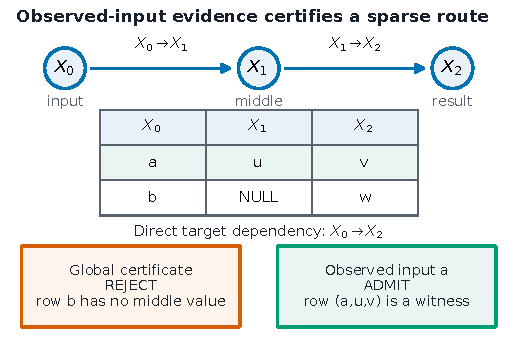
\includegraphics[width=\columnwidth]{figures/input_index_certificate_adjusted.pdf}
\caption{Observed-input certification of a globally rejected relational route.}
\label{fig:input-index-certificate}
\end{figure}
